\RequirePackage{luatex85}
\documentclass[border={20pt,20pt,20pt,20pt}]{standalone}

\usepackage[dvipsnames]{xcolor}
\usepackage{tikz}
\usetikzlibrary{shapes, patterns}

\begin{document}
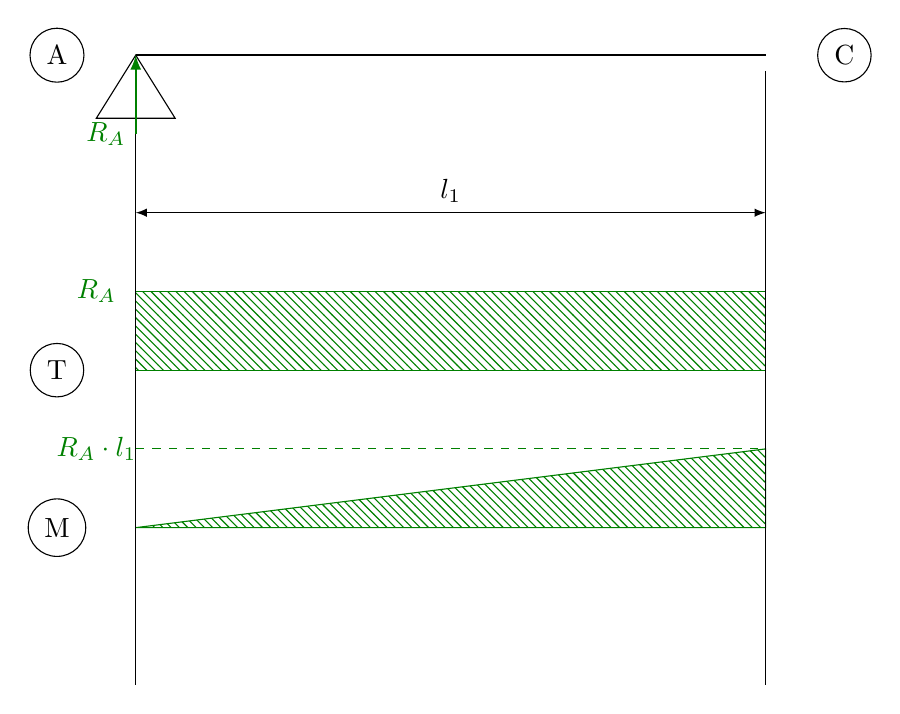
\begin{tikzpicture}[
	label/.style={circle,draw},
	gFill/.style={Green, pattern=north west lines, pattern color=Green},
	arrow/.style={latex-latex}
]
\draw[thick] (0, 0) -- (8, 0);
\node [label] at (-1, 0) {A};
\node [label] at (9, 0) {C};

\draw (0, 0) -- (.5, -.8) -- (-.5, -.8) -- cycle;

\draw [arrow] (0, -2) -- (8, -2) node[midway, above] {$l_1$};

% Tallant
\node [label] at (-1, -4) {T};
\draw (0, -4) -- (8, -4);
\draw[gFill] (0, -4) rectangle (8, -3);
\node[Green] at (-0.5, -3) {$R_A$};

% Moment
\node [label] at (-1, -6) {M};
\draw (0, -6) -- (8, -6);
\draw[gFill] (0, -6) -- (8, -5) -- (8, -6) -- cycle;
\draw[Green, dashed] (0, -5) -- (8, -5);
\node[Green] at (-0.5, -5) {$R_A \cdot l_1$};

\draw (0, -1) -- (0, -8);
\draw (8, -0.2) -- (8, -8);

\draw[-latex, Green, thick] (0, -1) -- (0, 0) node[at start, left] {$R_A$};
\end{tikzpicture}
\end{document}